\chapter{Preliminary Design}
\section{Design Specifications}
As a brief overview, the concept for the robot is to have a mechanically actuated eye mechanism with an integrated camera, which is mounted inside a ``head'', then attached to a ``body'' which is secured to attached to a rotating ``base''. These are the terms that will be used moving forward to refer to parts of the robot. The main functionality that the robot is demonstrating is face tracking. The robot, appropriately named Mr. I, will be able to maintain eye contact with the user. To accomplish this behavior, the robot will have three degrees of freedom, two for pan and tilt of the eye, and one for the rotating platform. It could be argued that one of the degrees of freedom is redundant, since simple pan and tilt is enough to track a moving object around a fixed point such as a camera. However, this design seeks to expand on existing face tracking camera products by adding a body to the camera. Not only does this give the robot more of a physical presence, but it also makes the motion of the robot more natural. When humans look at an object, they move their head first, then point their body towards the object. If the robot simply rotated its whole body without moving the eye first, it would look stiff and unnatural. Therefore, this additional degree of freedom is not redundant, in that it serves the purpose of making the robot more inviting and realistic.

\section{Concept Art}
\begin{figure}[h]
    \centering
    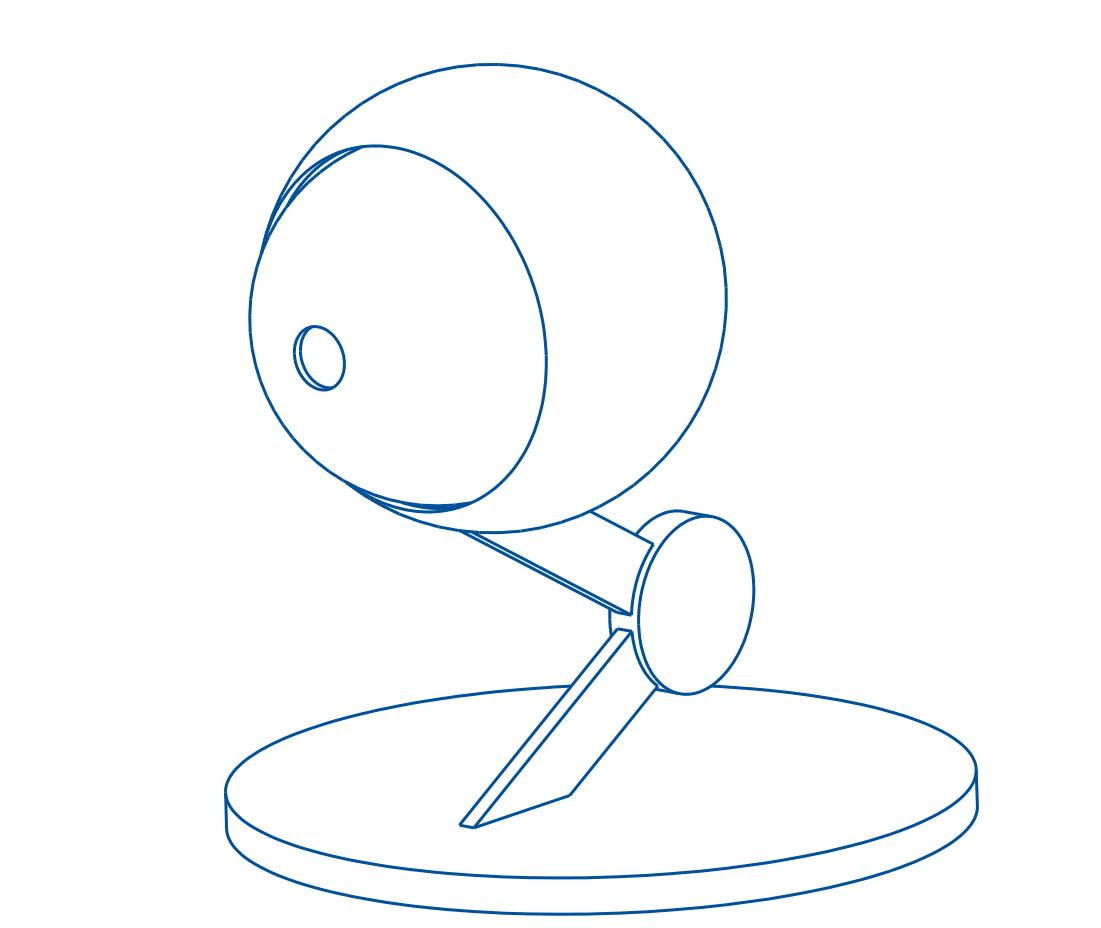
\includegraphics[width=0.5\linewidth]{Thesis/ch2/sketch.png}
    \caption{Initial Sketch}
    \label{fig:sketch}
\end{figure}
The earliest concept sketch is shown in Figure \ref{fig:sketch}. This was an idealized version of the robot with no mechanical components, but it laid the groundwork for the right proportions of the robot and outlined many of physical features that made their way into the final model. Notable features of this sketch are the eye mechanism being offset inside another sphere to act as the “head” of the robot, which would house the mechanical components and hide them for aesthetic purposes. Another thing to note is that the eyeball itself is a sphere with a small hole in the front for a camera see through. This was done to mimic the shape of a human eye, with the “pupil” being the camera hole. With the concept set, design work could then begin on the mechanisms.

\section{Eye Mechanism}
The first and most important part of the robot to be designed was the eye mechanism. The general concept for the eye mechanism was inspired by a project done by hobby content creator Will Cogley \cite{cogleyDIYCompact3D2019}. Cogley had created a video and Instructables post about his animatronic eye mechanism. Even more helpful was the fact that he open sourced the entirety of his design, including the model files and Arduino code. While none of the files themselves were used in this project, it was still a great reference and conceptual basis to build my project off of. One thing to note is that the project was a two-eyed mechanism, which would have to be cut down to one eye for this project. Most importantly, Cogley's mechanism does not incorporate a camera, nor does it accommodate it with the limited space in the small compact design. Cogley's project was on the scale of a normal human eye, but in order to fit a webcam into the eye the entire mechanism had to be redesigned from scratch to scale up the design and make it work for this application.

To explain the concept behind the eye mechanism, we can first start with the eye part itself. This is part we are trying to move, since it houses the camera. It is a sphere that rotates around its center point. Rotation about the center of a sphere can be defined in two parameters, which can be referred to as pan and tilt. These move the image camera in the x direction and y direction, respectively. As such, any parts moving the camera in the x-direction from this point forward will be given an ``x-'' prefix, and the same shall apply for parts that move the camera in the y direction.

\begin{figure}[h]
    \centering
    \begin{subfigure}[b]{0.475\textwidth}   
            \centering 
            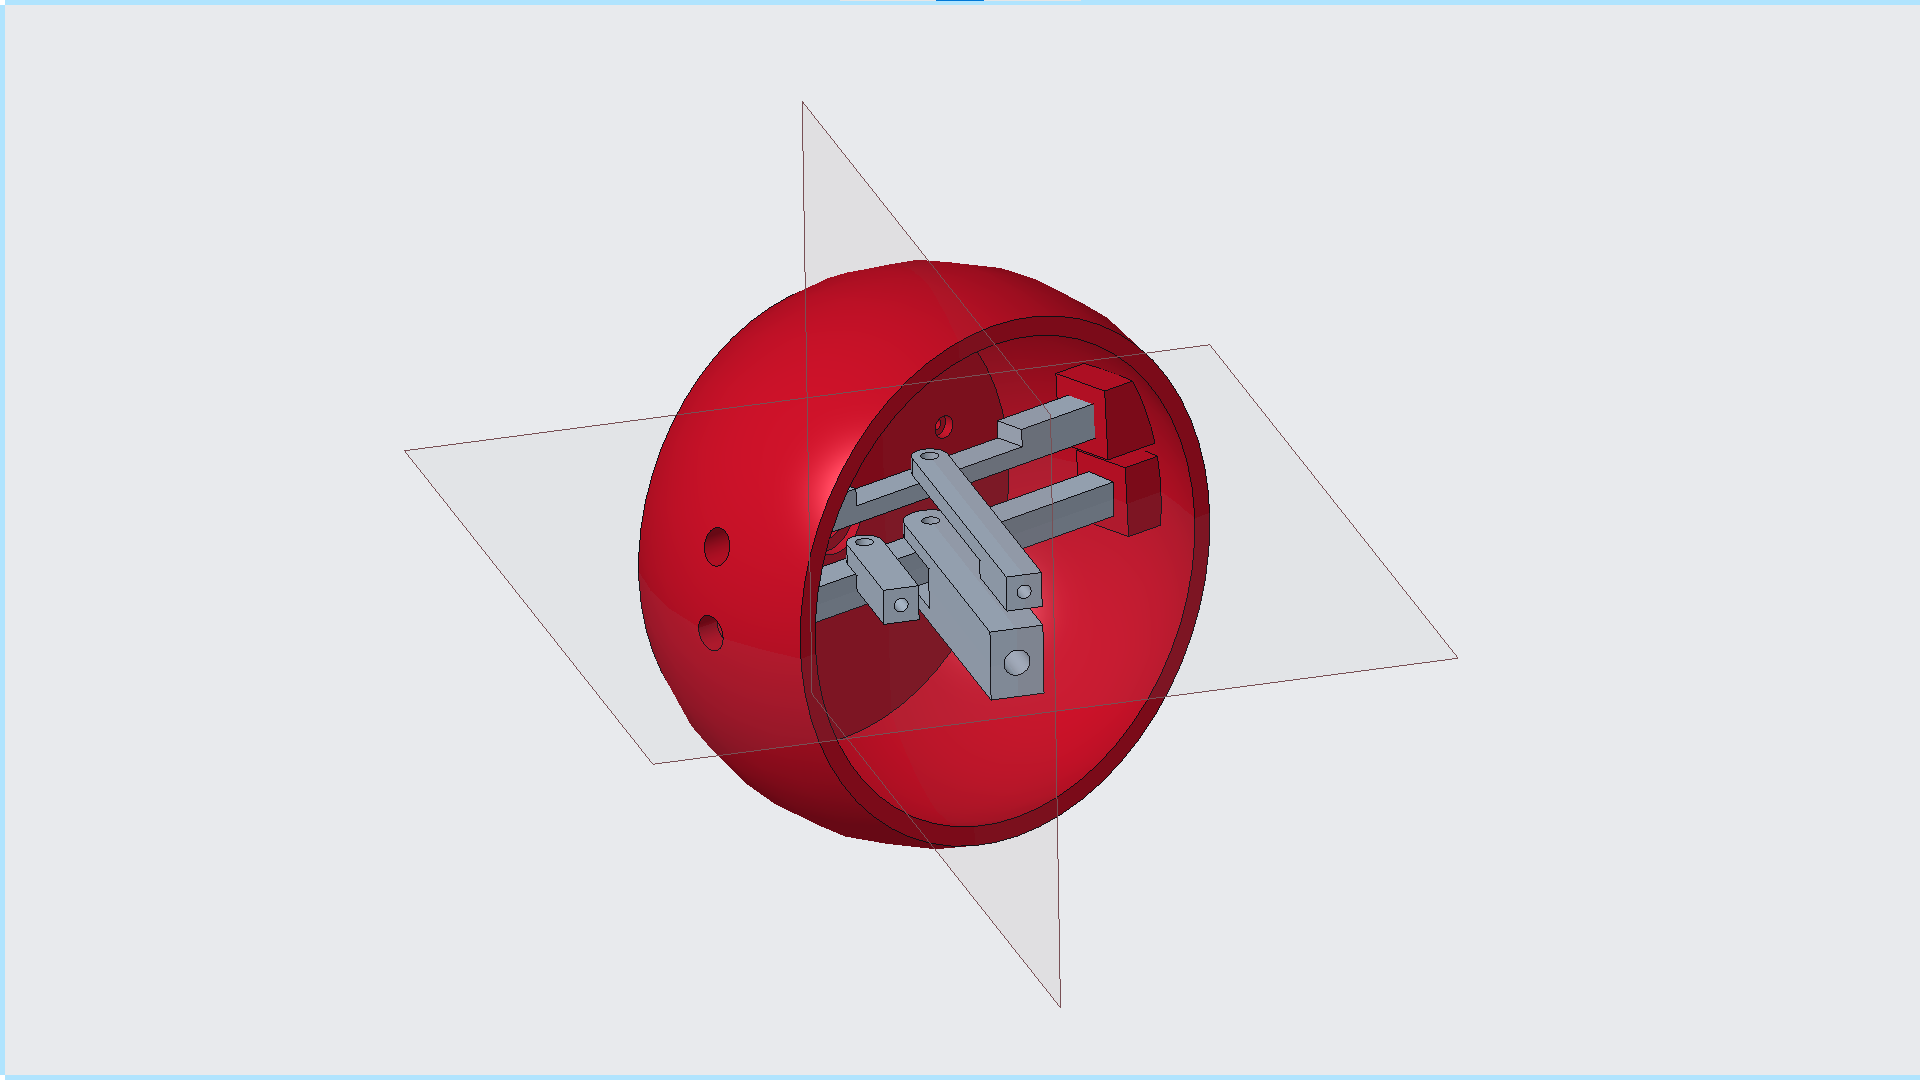
\includegraphics[width=\textwidth]{Thesis/ch2/left.png}
            \caption[]%
            {{\small Looking left}}    
            \label{fig:left}
    \end{subfigure}
    \hfill
    \begin{subfigure}[b]{0.475\textwidth}   
        \centering 
        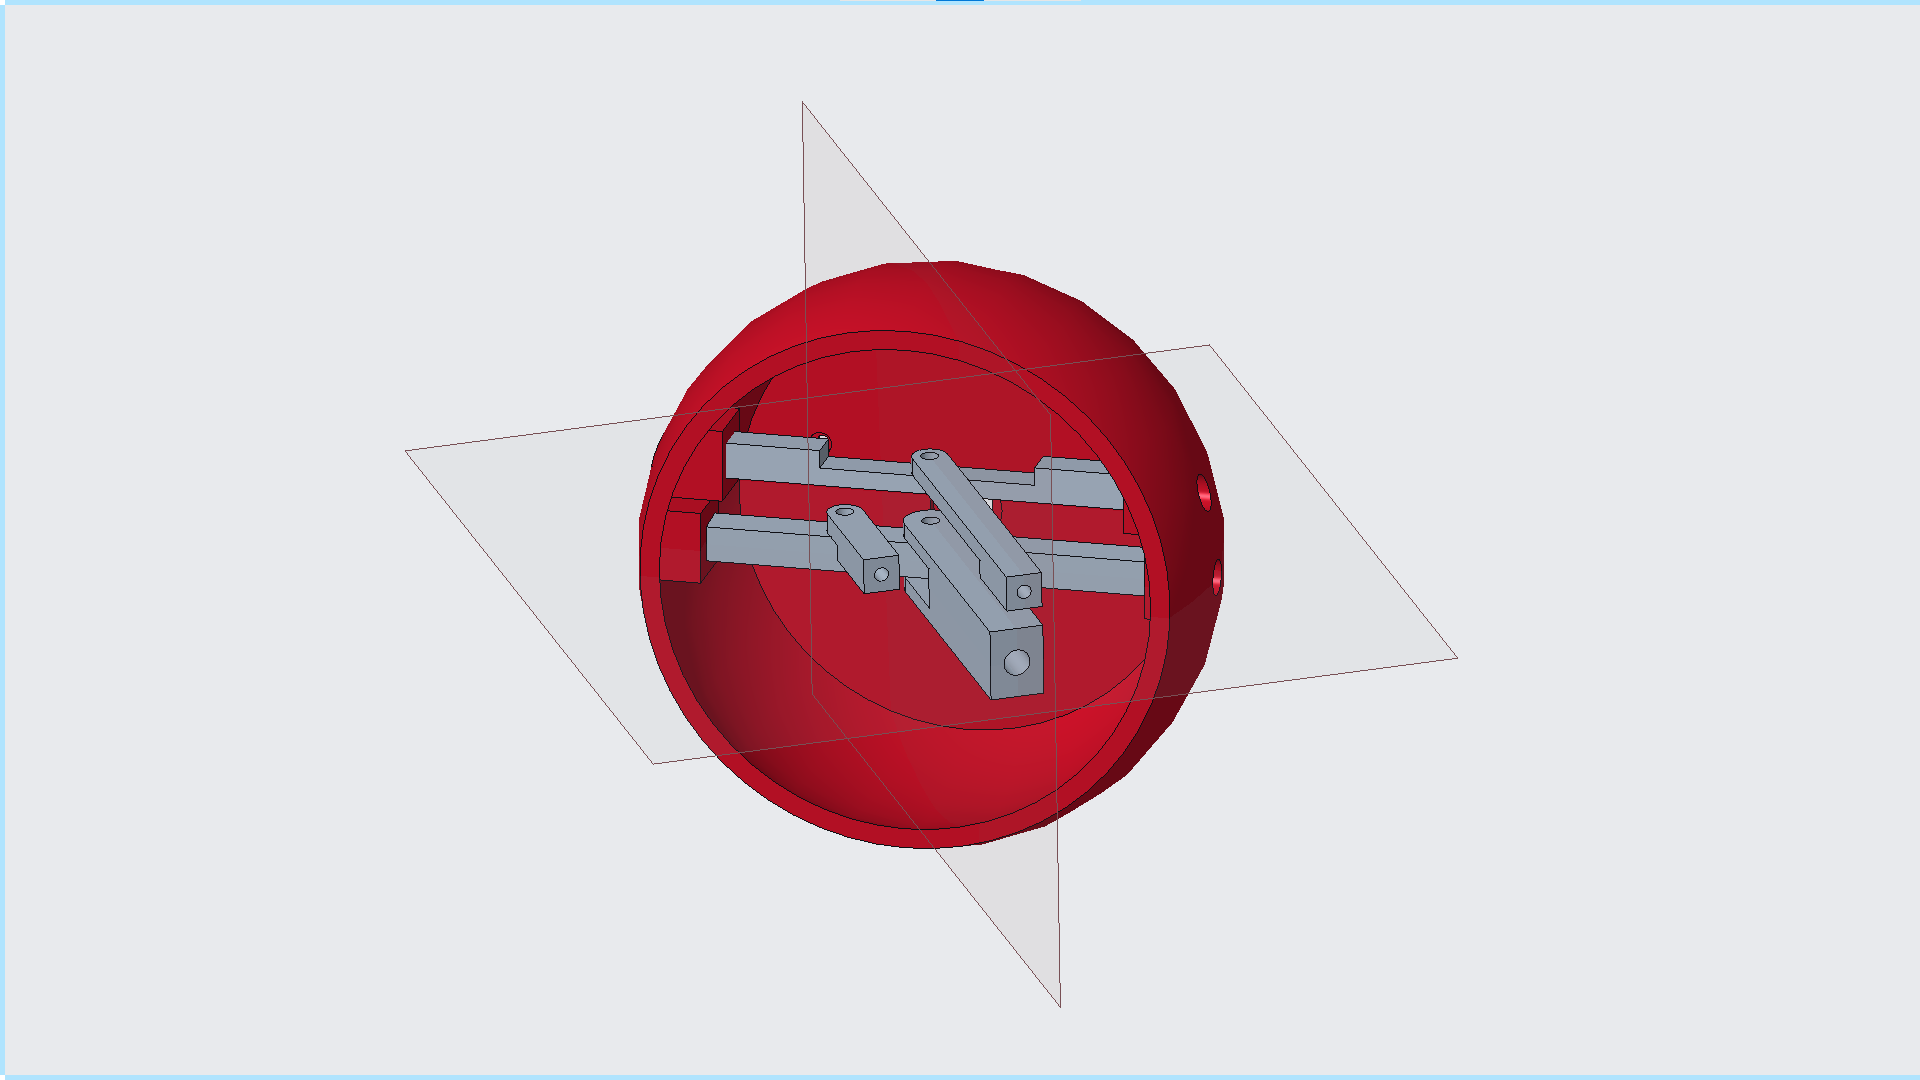
\includegraphics[width=\textwidth]{Thesis/ch2/right.png}
        \caption[]%
        {{\small Looking right}}    
        \label{fig:right}
    \end{subfigure}
    \vskip\baselineskip
    \begin{subfigure}[b]{0.475\textwidth}
        \centering
        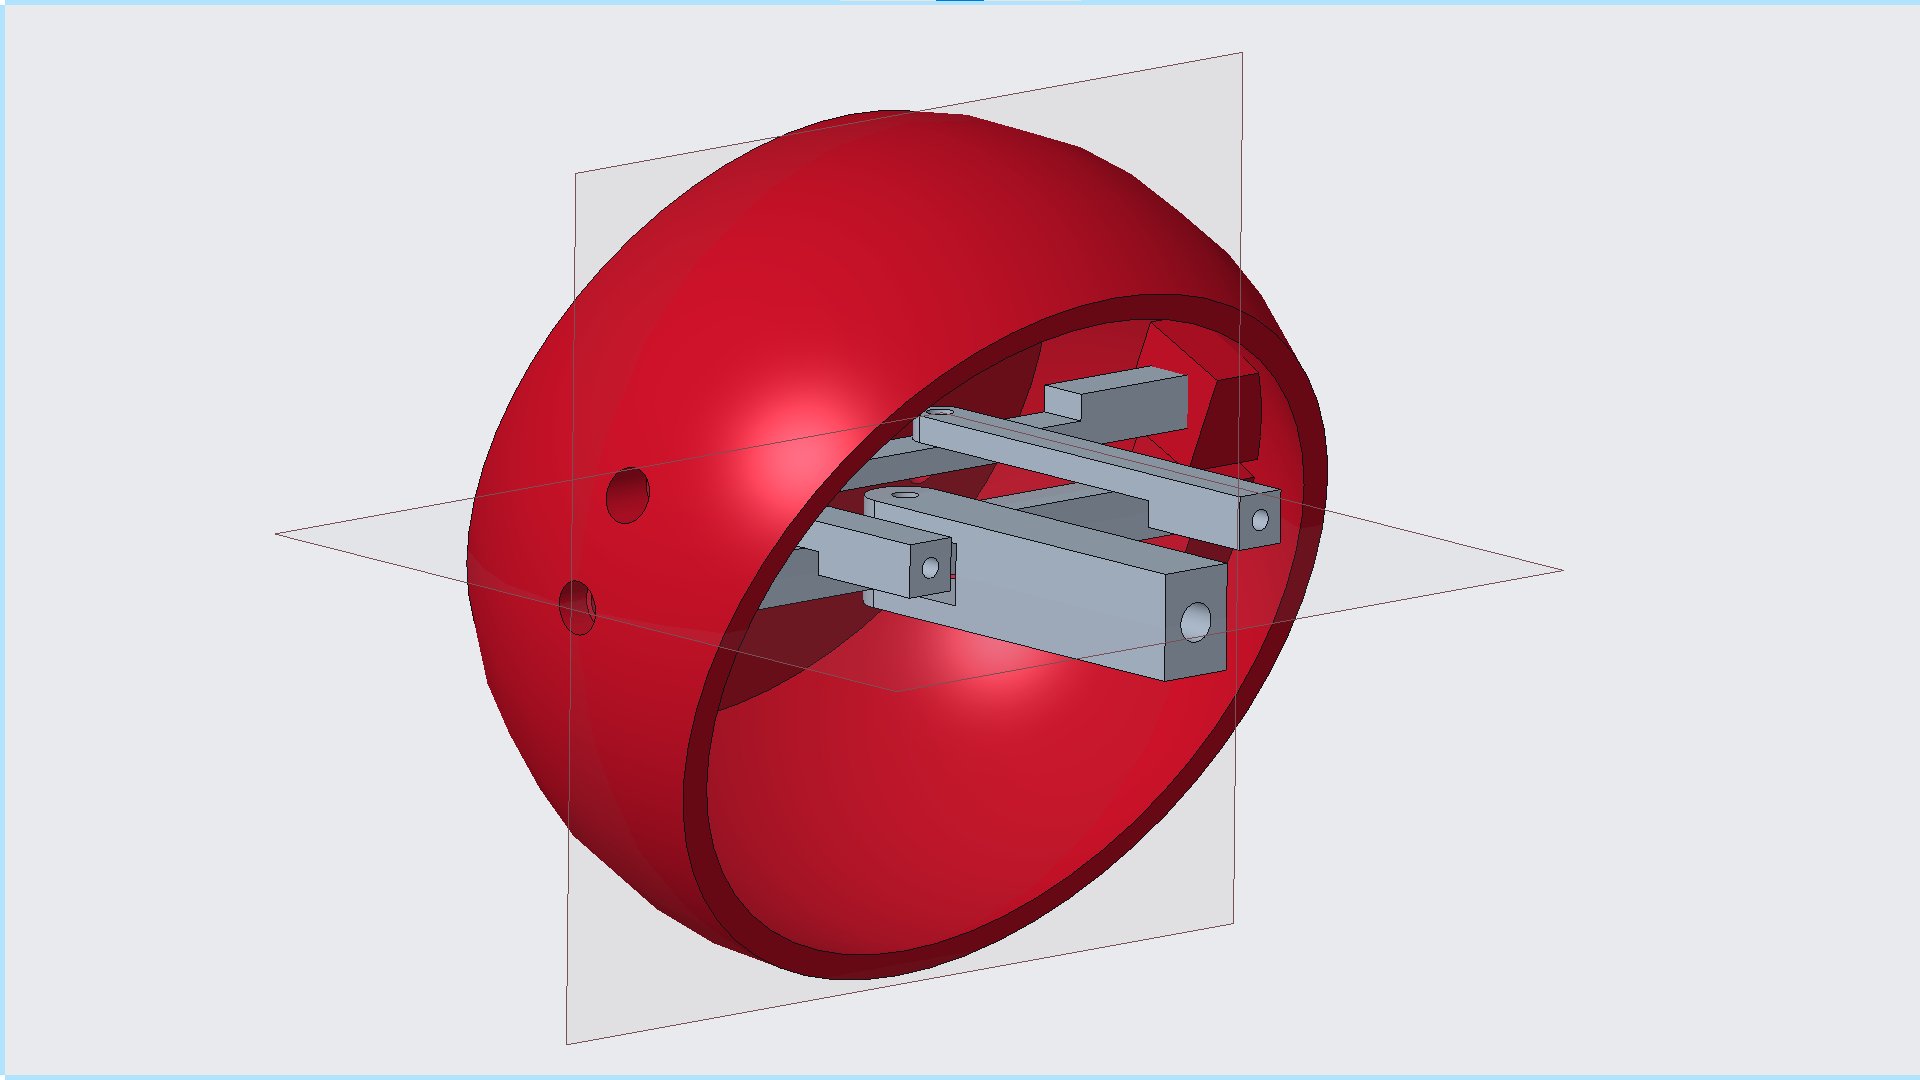
\includegraphics[width=\textwidth]{Thesis/ch2/top-up-2.png}
        \caption[]%
        {{\small Looking up}}    
        \label{fig:top-up}
    \end{subfigure}
    \hfill
    \begin{subfigure}[b]{0.475\textwidth}  
        \centering 
        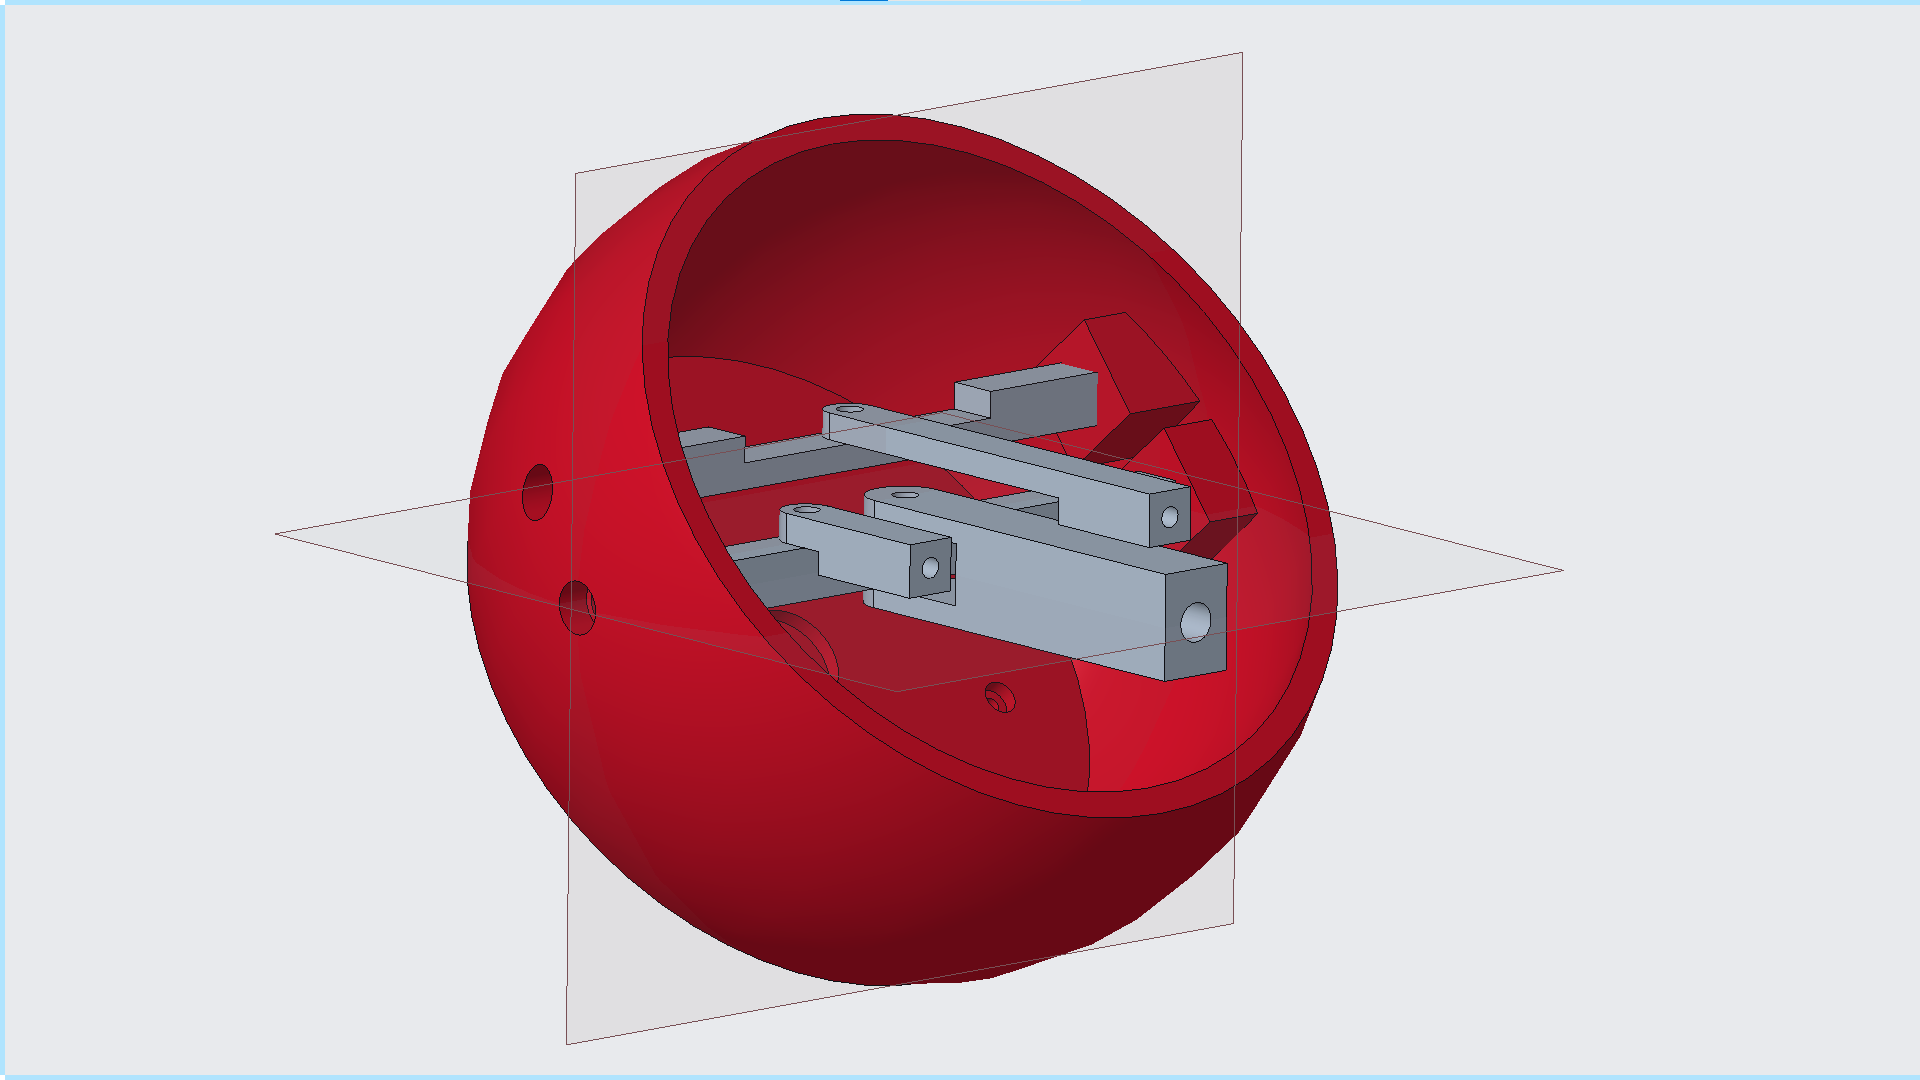
\includegraphics[width=\textwidth]{Thesis/ch2/top-down.png}
        \caption[]%
        {{\small Looking down}}    
        \label{fig:top-down}
    \end{subfigure}
    
\caption{Basic movement behind the eye mechanism.}
\label{fig:eye-mech}
\end{figure}
The x-motion of the eye is relatively trivial to implement. The eye can simply be attached to a horizontal support, called the x-support, and the support is attached via a pin joint at its center to a main support. Any pushing motion on the x support would exert a torque and pan the camera left and right. This is seen in Figures \ref{fig:left} and \ref{fig:right}. The y-motion is accomplished by adding a second support above the x-support. By attaching both supports to the eye part with pin connections, this affords the eye part the extra degree of freedom to tilt up and down as well. This tilting motion can be controlled by exerting a torque on the eye part itself by pushing the y-support forwards and backwards with a linkage connected in the center of the support, shown in Figures \ref{fig:top-up} and \ref{fig:top-down}. The key to making the mechanism work is that the pin joints afford the eye enough degrees of freedom such that the x and y directions can be controlled independently of one another. The moment arms of the x and y linkages intersect at the center of the circle, so motion in the x and y direction can be accomplished by simply pushing their respective supports. This simple motion can be accomplished by two basic servos. A full video animation demonstrating this behavior can be found in Appendix \ref{ch:videos}.

\subsection{Design Iterations}
\label{ch:design-iterations}
\begin{figure}[h]
    \centering
    \begin{subfigure}{0.4\linewidth}
        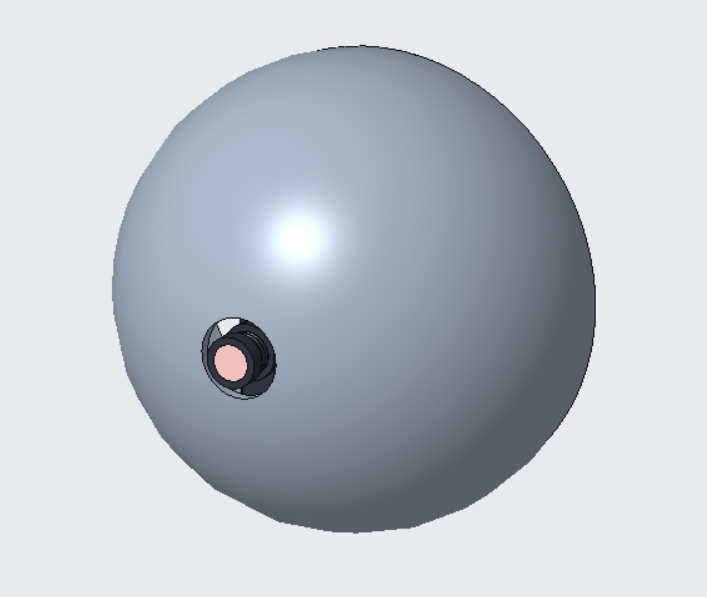
\includegraphics[height=2in]{Thesis/ch2/first-iteration.png}
    \end{subfigure}
    \begin{subfigure}{0.4\linewidth}
        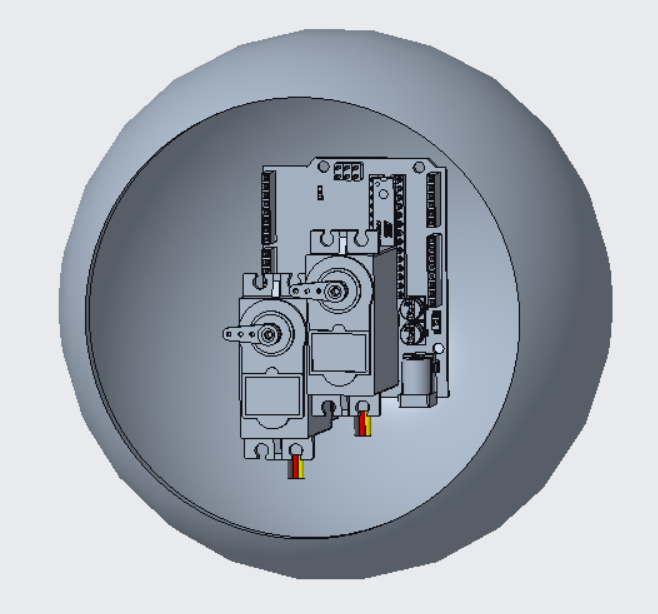
\includegraphics[height=2in]{Thesis/ch2/first-iteration-2.png}
    \end{subfigure}
    \caption{First iteration.}
    \label{fig:first-iteration}
\end{figure}

The oldest saved draft of the eye mechanism is shown in Figure \ref{fig:first-iteration}. At this early stage, an Arduino Uno was planned to be used as the microcontroller for the project, along with two HS-645MG servos, which are common servo motors used in hobby projects. These servos in particular were chosen for their impressively high torque for their size, a standard 40x40x20mm. At this early stage, higher torque motors were desirable for safety margins, especially since the rest of the mechanism had not been designed yet, but in the end these servos proved to be a wastefully expensive choice. The final servos used were half the price and had the same form factor, so it did not require much refactoring of the design; it was a drop in replacement. Another component that went through some changes was the camera. In this early stage, an ArduCam was planned to be used, as it is able to connect up directly to the Arduino. However, after further research it was concluded that the Arduino chip is not powerful enough to run the computer vision algorithms required to achieve face tracking, so this part was changed to a USB webcam to easily be able to interface with a laptop. The Logitech C615 USB Webcam was chosen for this purpose because of its low price and compact design, as well as being 1080p. This higher resolution would help in the computer vision developed later on. The webcam incorporated into the eyeball can be seen in Figure \ref{fig:iteration2}.

\begin{figure}[h]
    \centering
    \begin{subfigure}{0.4\linewidth}
        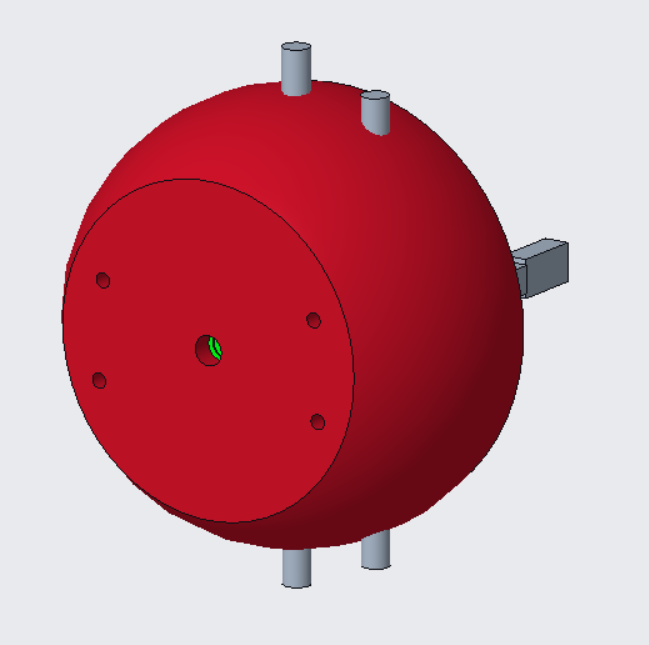
\includegraphics[height=2.2in]{Thesis/ch2/iteration2.png}
    \end{subfigure}
    \begin{subfigure}{0.4\linewidth}
        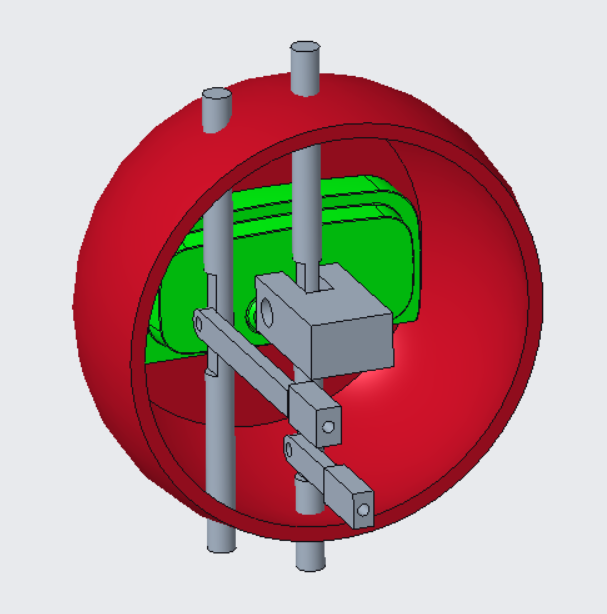
\includegraphics[height=2.2in]{Thesis/ch2/iteration2-2.png}
    \end{subfigure}
    \caption{Second iteration.}
    \label{fig:iteration2}
\end{figure}

After further design and some early 3D printing testing, one issue with the design was found: the cord for the camera was intersecting with the main vertical support. So, the entire design had to be rotated 90 degrees to put the linkages above the camera, since the cord was coming out of the bottom half of the camera. This is the orientation that is reflected in the final design today, shown in Figure \ref{fig:iteration3}

\begin{figure}[h]
    \centering
    \begin{subfigure}{0.4\linewidth}
        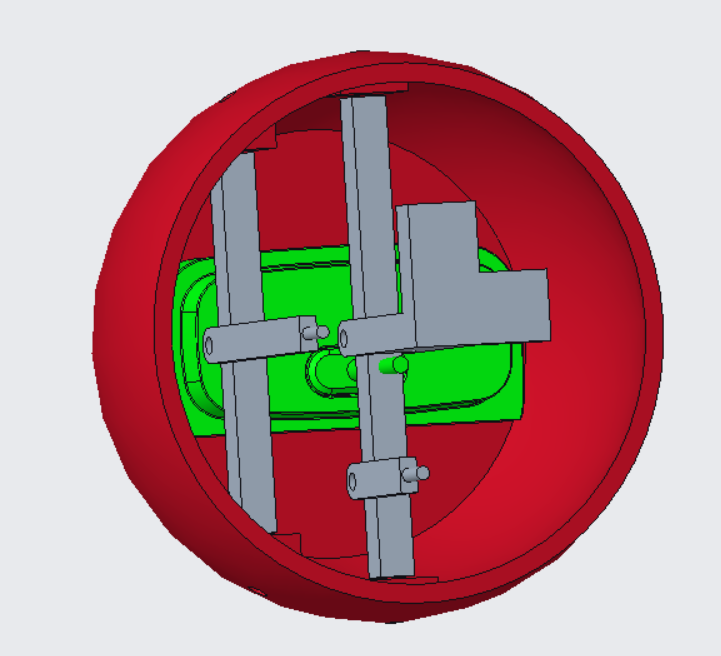
\includegraphics[height=2in]{Thesis/ch2/iteration3.png}
        \caption{Before}
    \end{subfigure}
    \begin{subfigure}{0.4\linewidth}
        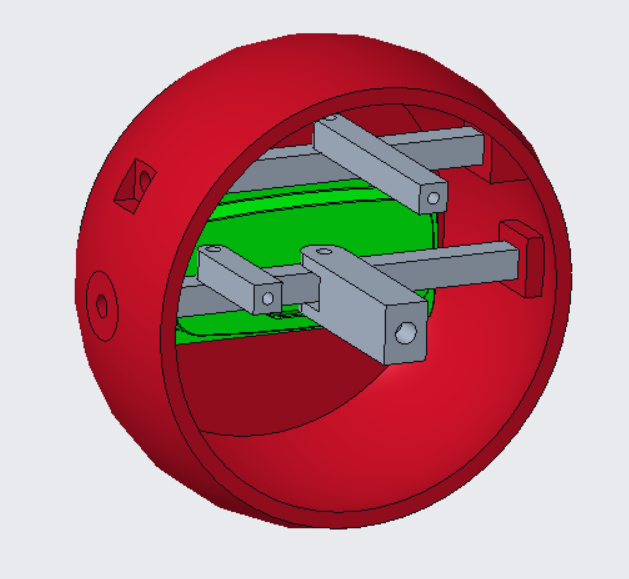
\includegraphics[height=2in]{Thesis/ch2/iteration3-2.png}
        \caption{After}
    \end{subfigure}
    \caption{Changes in the orientation of the eyeball.}
    \label{fig:iteration3}
\end{figure}


After this stage, servo motors were ready to be added in to supply the pushing motion needed to pan and tilt the eye part. One thing to note is that the servos had to be attached with ball linkages rather than pin joints. This is because the pushing motion of the eye linkages is not strictly one-dimensional. The y-linkage for instance moves slightly up and down as it rotates around the sphere of the eye part in addition to being driven forwards and backwards by the servo. For this reason, the ball joint was necessary to add some slack in the mechanism to account for this slight up and down movement. This was not necessarily required for the x-servo, as its motion is completely in line with the servo arm, but a ball joint was still used to accommodate any manufacturing defects or misalignments.
Since this prototype was done before the rest of the head and robot were designed, a temporary mounting block was modeled and mounted to a piece of scrap metal just to get something up and running quickly. This was named as the first working prototype of the eye mechanism, shown in Figure \ref{fig:first-prototype}.

\begin{figure}[h]
    \centering
    \begin{subfigure}{0.48\linewidth}
        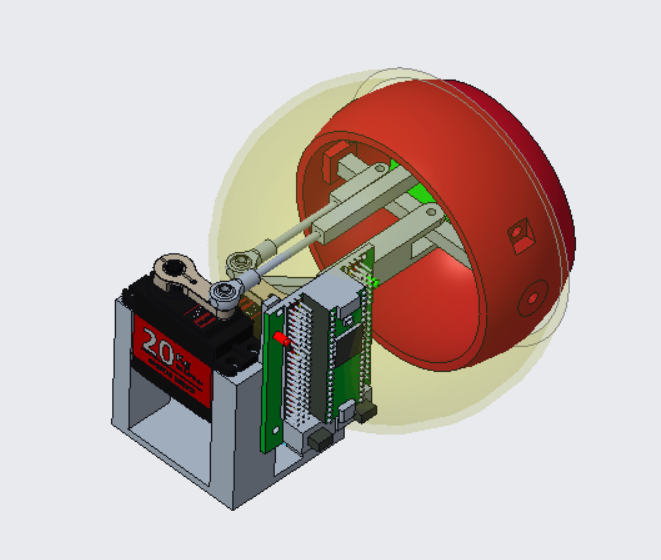
\includegraphics[width=\textwidth]{Thesis/ch2/first-prototype.png}
    \end{subfigure}
    \hfill
    \begin{subfigure}{0.48\linewidth}
        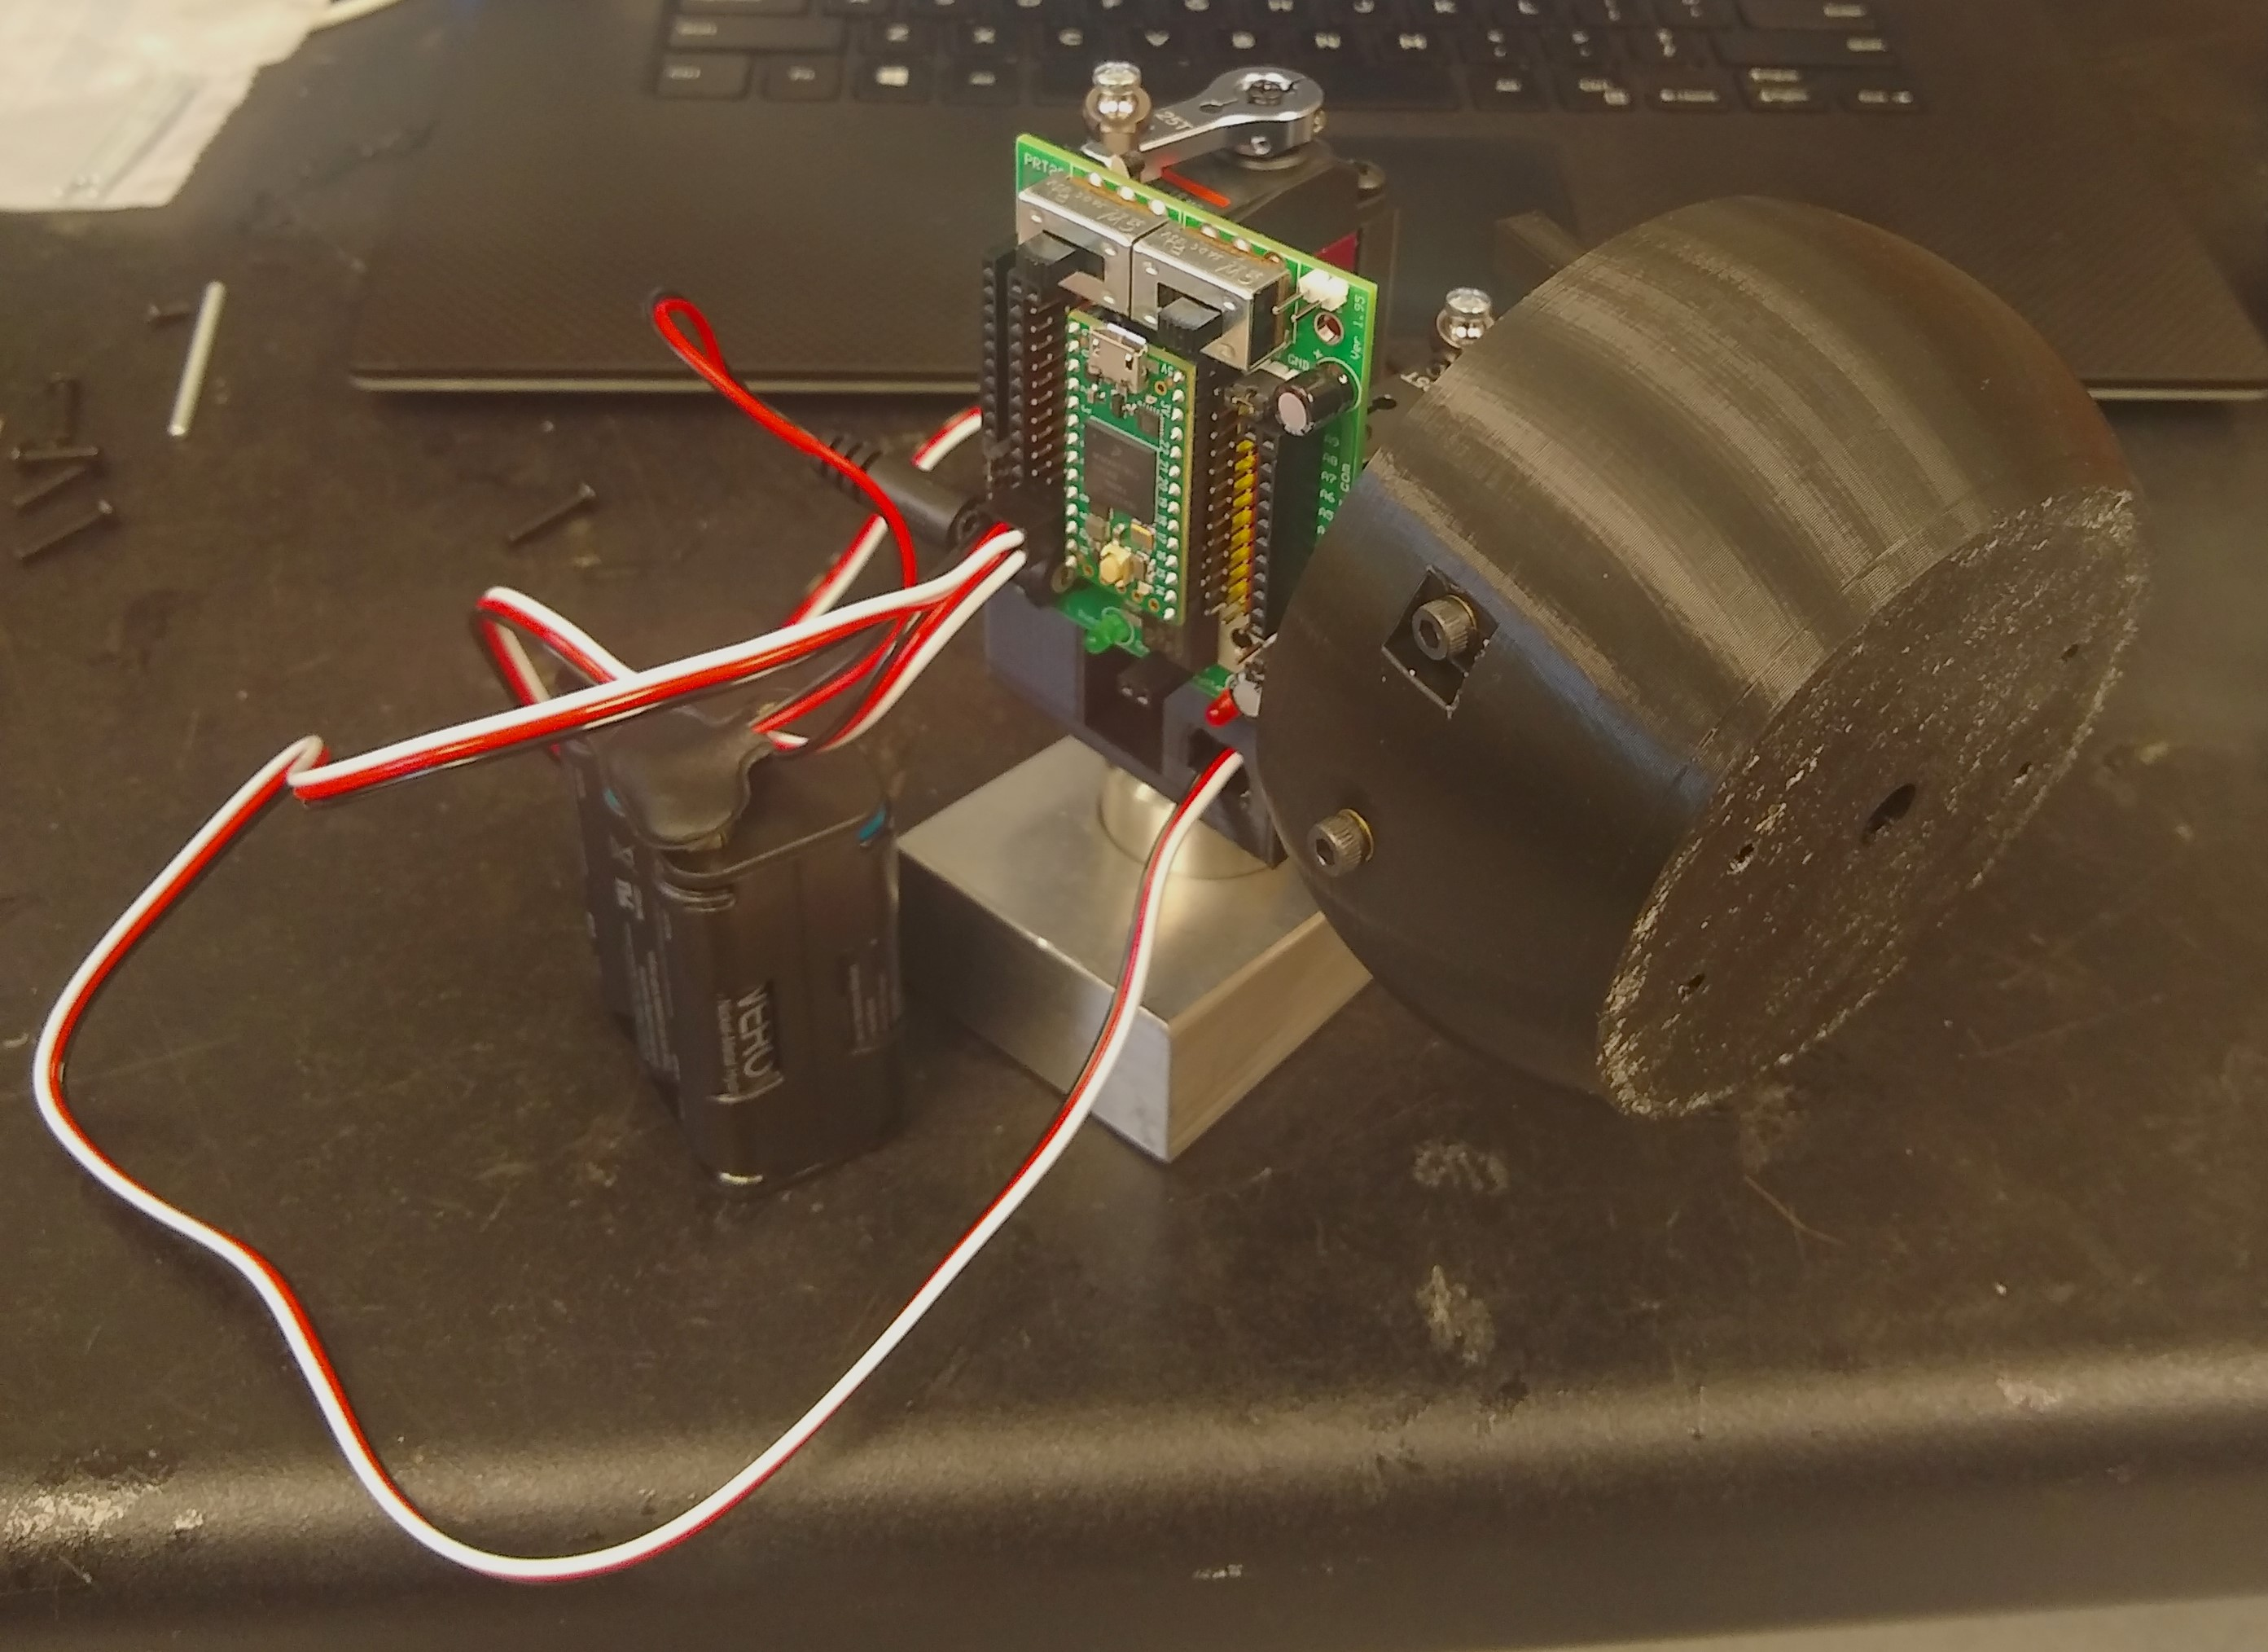
\includegraphics[width=\textwidth]{Thesis/ch2/first-proto-cropped.jpg}
    \end{subfigure}
    
    \caption{First working prototype.}
    \label{fig:first-prototype}
\end{figure}

In this prototype, a simple Arduino script was used to cycle the eye through looking through 8 directions, up down left and right and diagonals. The diagonals were to test the independence of the x and y controls, which was successful. A video of the first prototype moving can be seen in Appendix \ref{ch:videos}. This prototype was powered with a Teensy 4.0 microcontroller \cite{pjrcTeensy2023}, which is interfaced with a motherboard designed by Patton Robotics \cite{pattonPRT28Patton2018}. This board allows for the board to be powered by an external power source, in this case a 6 AA battery pack. The board features a voltage regulator to step down the 9V battery source to a useable 5V for the servos and microcontroller. For this reason, this microcontroller and motherboard combination was used all the way into the final design. 

One shortcoming identified in this stage was the range of motion of the eye. Previously the eye linkages were placed towards the outside of the eye sphere, as it would increase the moment arm of the servos and allow them to exert a greater torque on the rotating eye. However, testing showed that this greatly reduced the eye's range of motion, as the back of the eye would intersect with the linkages. The initial test also showed that the torque required was much smaller than planned, since the servos are simply rotating the eye, which requires less force than translating it. As such, the linkages were then moved as close to the center as possible while leaving clearance for all the fasteners and support beams. To accomplish this, the linkages were made more slender and incorporating notches in the bars so that the linkages could rotate within the supports rather than on top of them. The parts of the beams outside the notches were thick enough to provide structural stability to the eye mechanism. These optimizations reduced the material costs of the parts and made the design as compact as possible.

\section{Head}
The head of the robot is the part that surrounds the eye mechanism. This is to protect the mechanism from dust and debris, protect the user from getting caught in the moving parts, and also give the robot a better aesthetic look. The head consists of four plates that form a sphere around the eye mechanism. The motor mounting block has multiple protrusions that provide attaching surfaces for the plates. This is shown in Figure \ref{fig:head-diagram}. The top two plates were designed to be secured with neodymium magnets to be easily removed for inspecting and servicing the inner mechanism. The magnets are not strong enough to hold the bottom plates upside down, so the bottom plates are screwed in to secure them but still allow for disassembly. 

\begin{figure}[h]
    \centering
    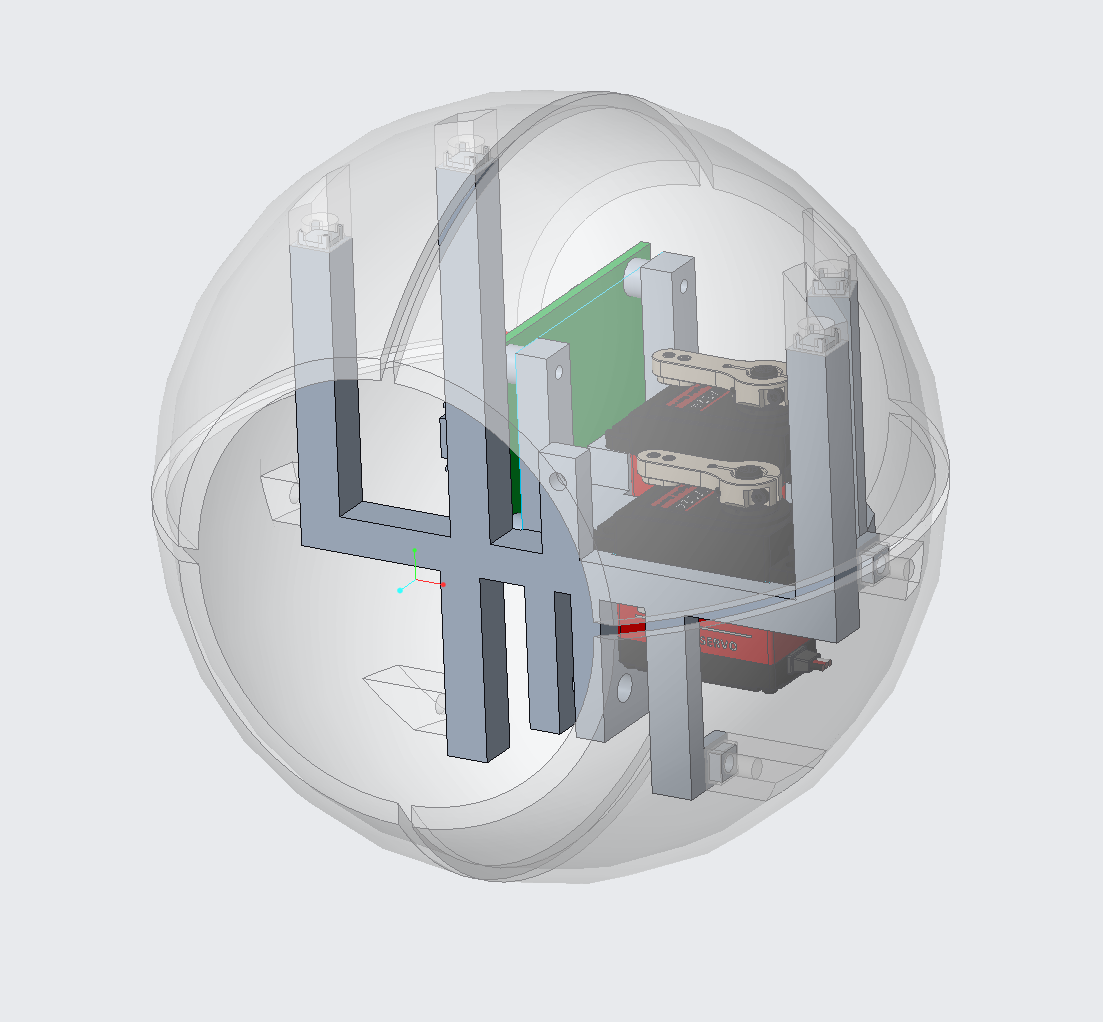
\includegraphics[width=0.5\linewidth]{Thesis/ch2/head-diagram.png}
    \caption{An inside look at the head assembly.}
    \label{fig:head-diagram}
\end{figure}

\section{Body}
The body of the robot is the part that connects the head to the base. The head is secured to the body via a mounting feature in the motor mount that straddles the body, then secures it in place with two screws. The early design for the body was planned to have multiple parts and have a more acute angle. The idea behind the bend was to model a person bending over, as this would give the body a more human-like shape than a straight line. However, it was found that the initial sketch looked unnatural as it was too bent over. The figure below shows the change in angle that produced a much more natural body shape that made it into the final model.
\begin{figure}[h]
    \centering
    \begin{subfigure}{0.4\linewidth}
        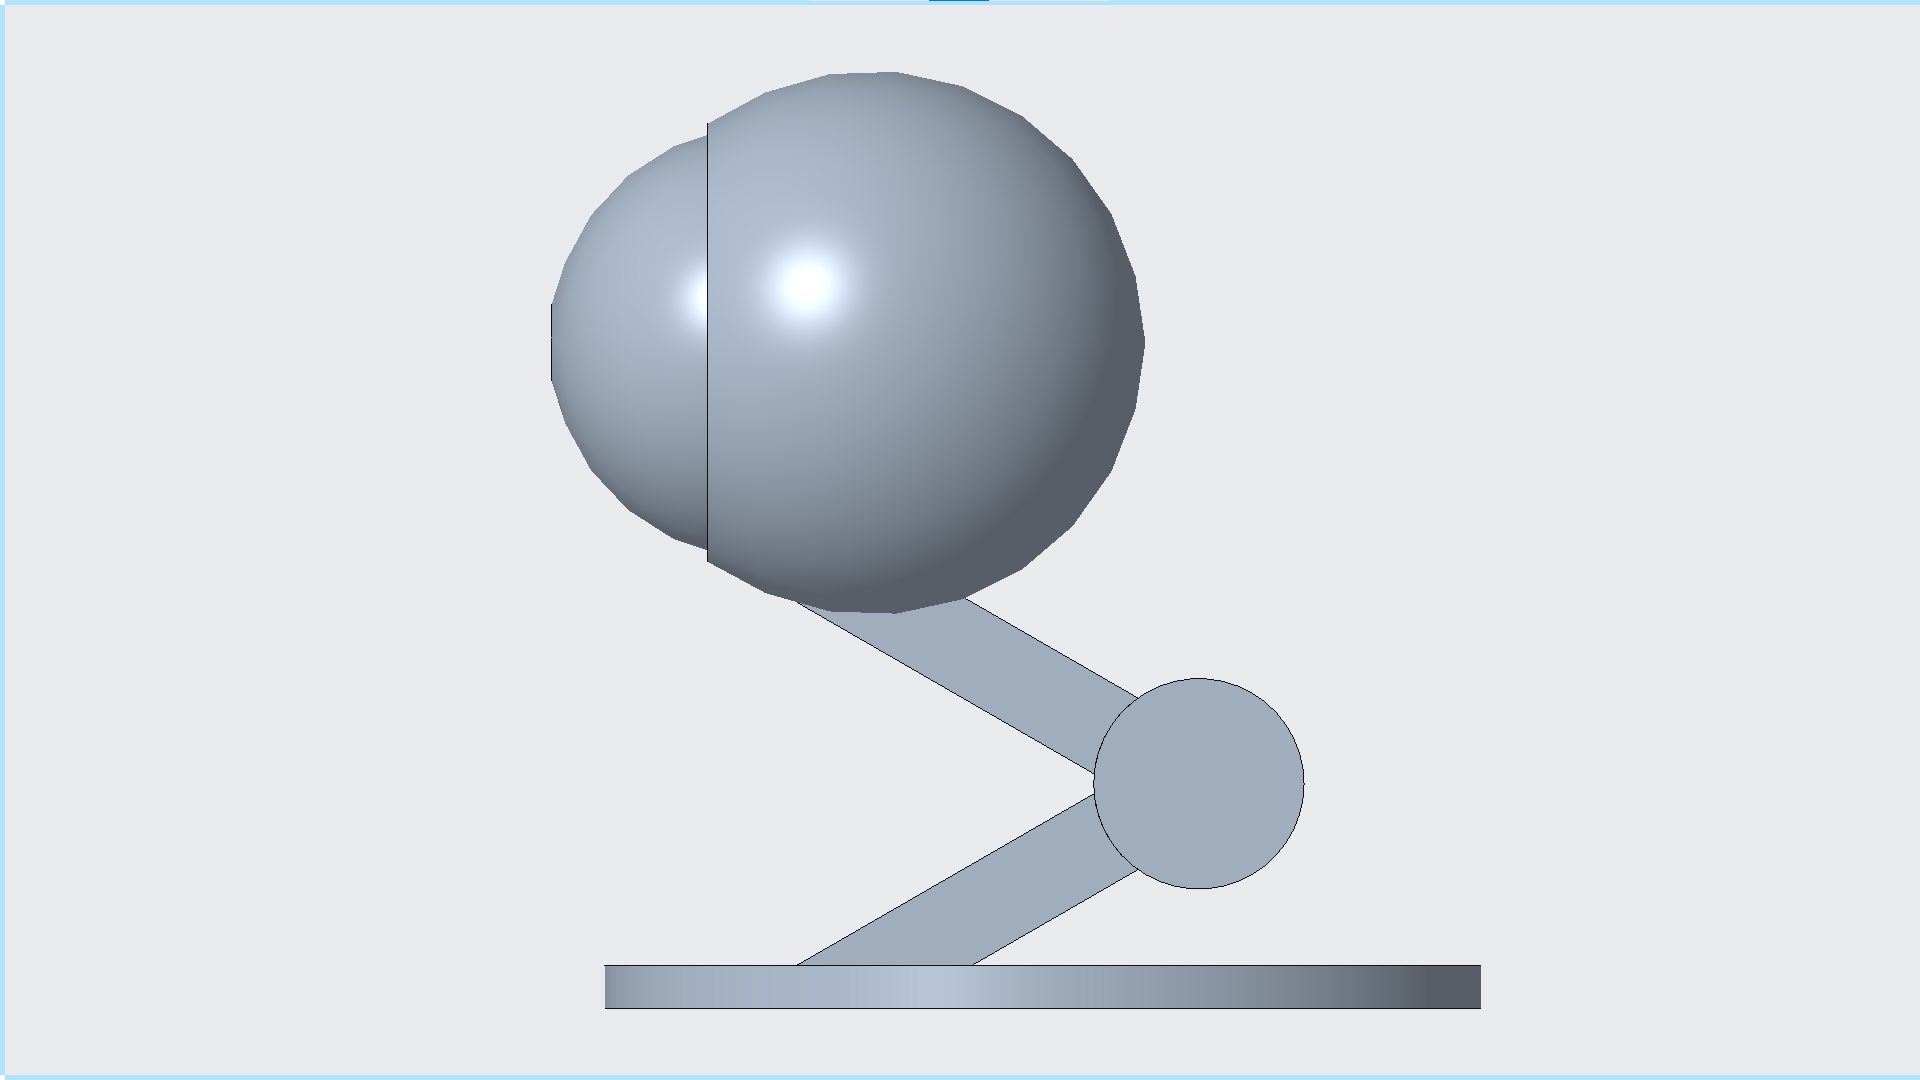
\includegraphics[width=\linewidth]{Thesis/ch2/side-view2.png}
        \caption{Before}
    \end{subfigure}
    \begin{subfigure}{0.4\linewidth}
        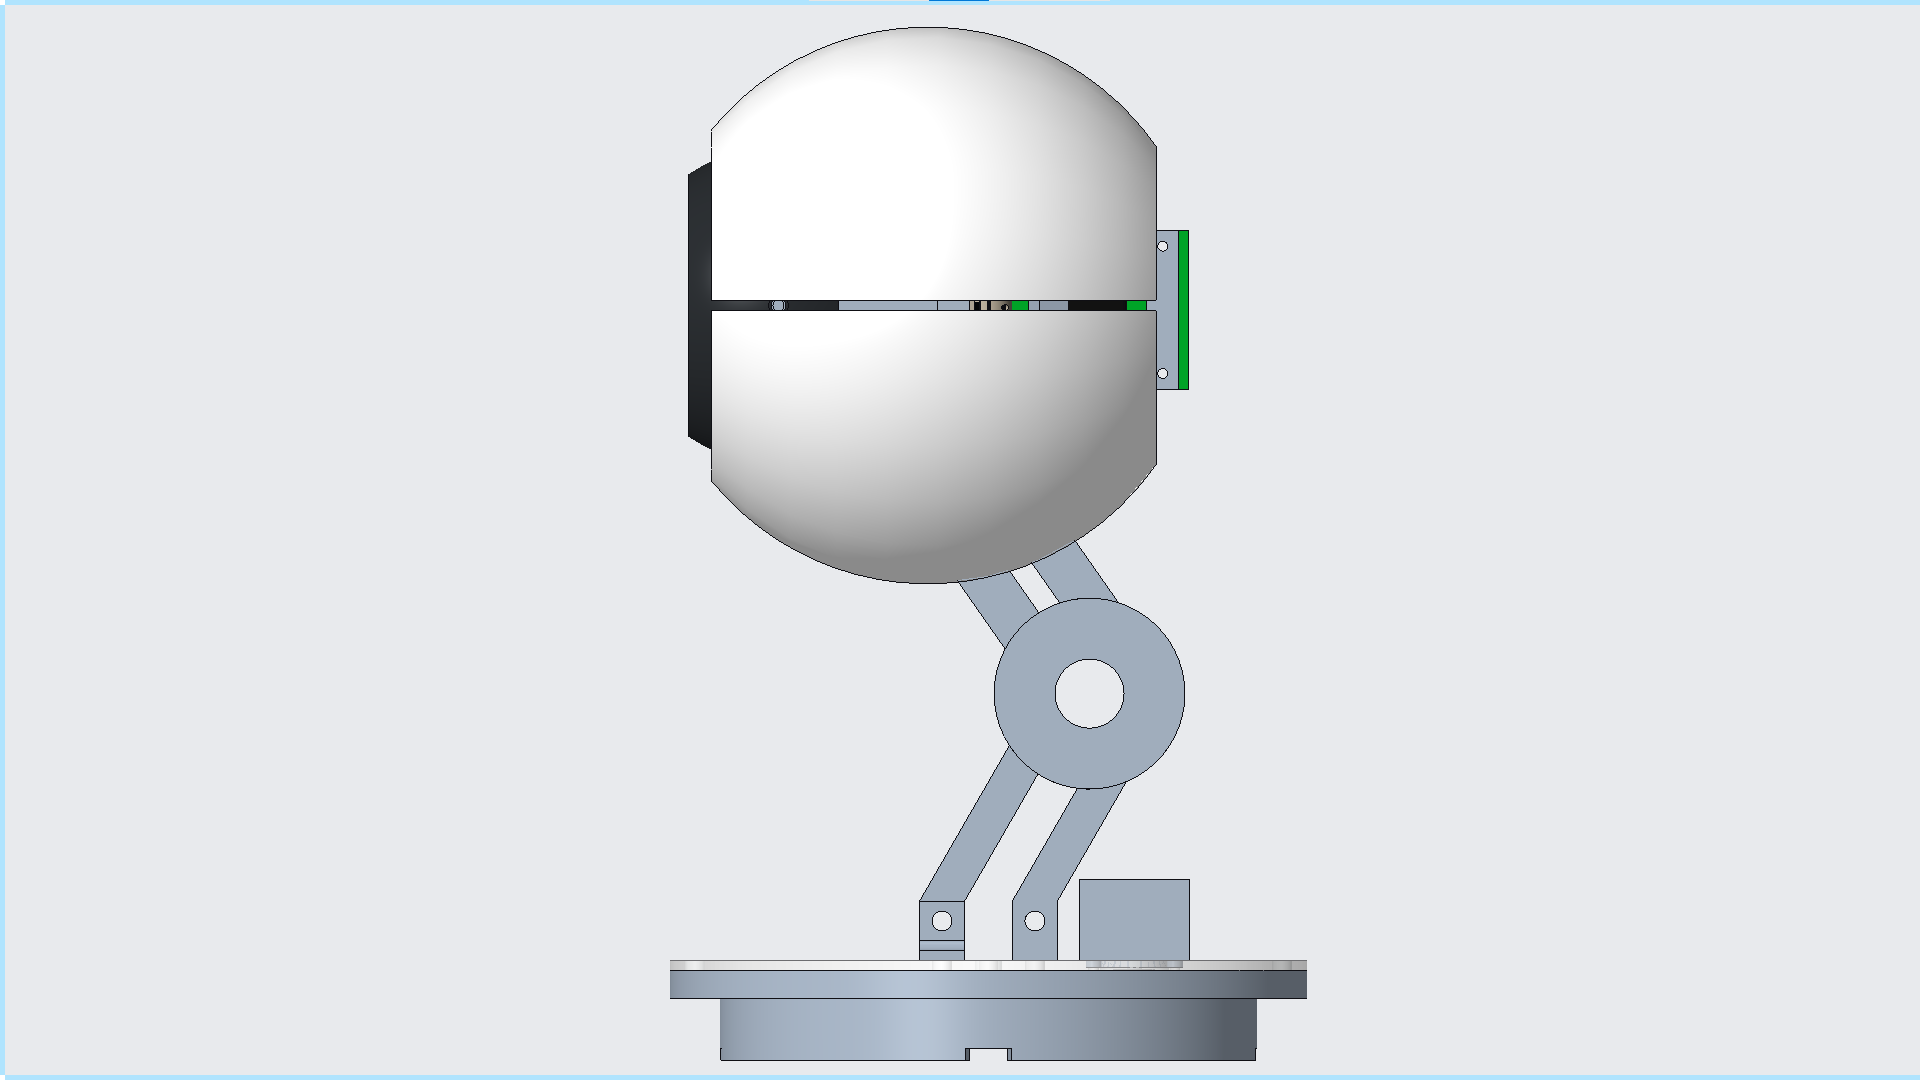
\includegraphics[width=\linewidth]{Thesis/ch2/side-view1.png}
        \caption{After}
    \end{subfigure}
    \caption{Comparison of the shape of the robot body.}
    \label{fig:body_comparison}
\end{figure}

\section{Base}
The base of the robot is what allows the robot to stand on a surface by itself. The base had to be large enough such that it would provide enough lateral stability to keep the robot from tipping over. The base also allows the robot to rotate $360^\circ$, as outlined previously. The base is divided into two sections, the top half being connected to the rest of the robot and the bottom half that is stationary. A stepper motor was used to rotate the top half of the base, which in turn would rotate the rest of the robot. The stepper motor is attached to the top half of the base. The motor is mated with a gear that interfaces with an internal gear modeled around the bottom half of the base. This internal gear mechanism drives the third and final axis of the robot.

Gears incorporated in the base were obtained from step files from McMaster-Carr \cite{MetalGear20}\cite{MetalInternalGear} and scaled and modified to fit this application. The original inner and outer gears had pitch diameter of 0.5 in and 3.00 in respectively, yielding a gear reduction ratio of 1:6. This ratio was chosen because the motor chosen was relatively small, but capable of very fast speeds. The gear ratio was chosen to be low enough to gear down the speed and increase the torque of the motor, while also keeping the gears large enough to be 3D printed with reasonable accuracy. The STEP files obtained from McMaster-Carr were scaled up by a factor of \(\frac{11}{6}\) to fit in the model.

Additionally, it was planned to have a slip ring in the center to allow for continuous rotation of the base, shown in Figure \ref{fig:slipring_sketch}. This idea was tested but it was found that the slipring was not reliable enough to transmit camera signals over USB. The way a slipring works is it has brushes that make contact with metal inside the slipring as it rotates. This allows it to keep electrical contact but rotate freely. Otherwise, if there were solid wires, they would get wrapped up in each other. However, these brushes are not perfect, and ideally there is always some brushes making contact but for a small instant they may not be making contact. This is fine for a low frequency signal but USB is high bandwidth. Moreover, a camera needs to send a lot of information over USB. This makes it catastrophic if even a single bit of information is lost. It was found that the camera was able to be routed through the slipring but once the slipring rotated even a little bit, the camera feed was distorted and disconnected from the PC. This idea was scrapped from the project, instead constraining the motor to rotate $180^\circ$ in either direction for a full $360^\circ$ range of motion. However, this was actually did not have an impact on the functionality of the robot since it can be assumed that the user will not be constantly encircling the robot while having a conversation with it. If the robot is on a table against a wall for instance, there will never be a time where it needs to make a $360^\circ$ rotation, let alone multiple.

\begin{figure}[h]
    \centering
    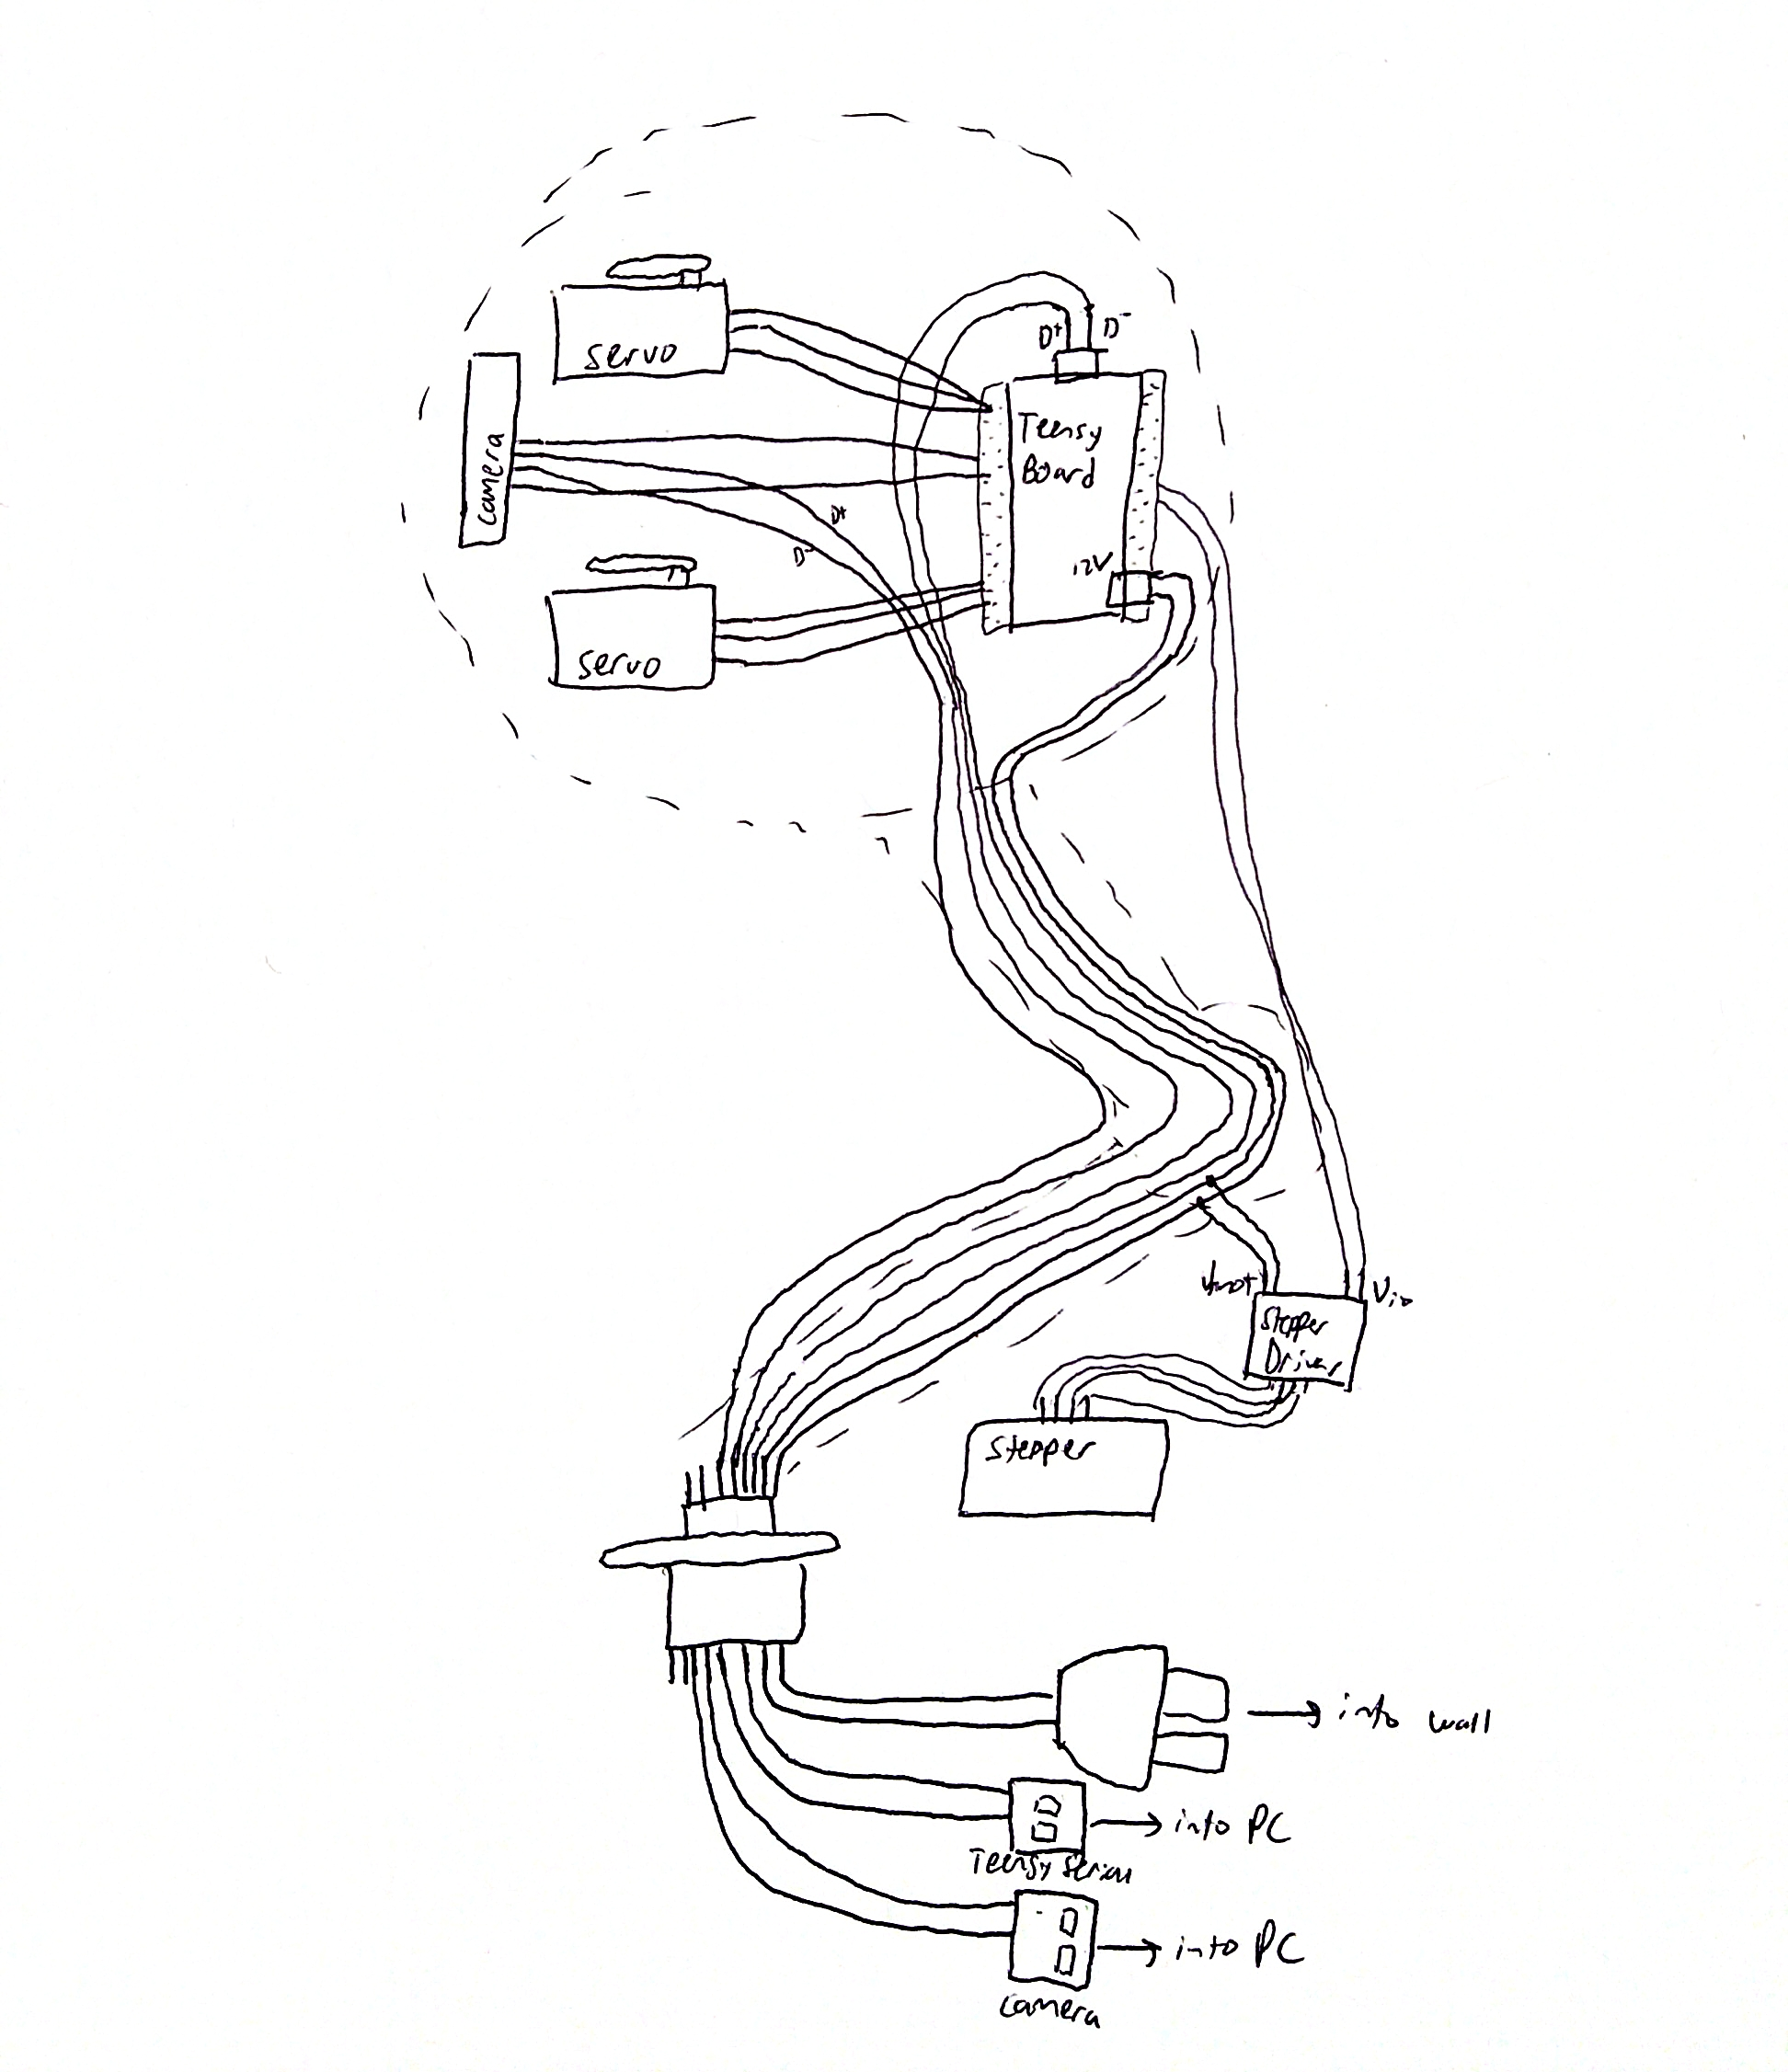
\includegraphics[width=0.5\textwidth]{Thesis/ch2/Document 25_2.jpg}
    \caption{Early slipring sketch that was scrapped.}
    \label{fig:slipring_sketch}
\end{figure}


\subsection{Analysis}
A mechanism analysis was performed in Creo to determine the proper placement of the eye in relation to the head and where to place the linkages to get away from the eye. Instead of being constrained as a fixed part, the eye part could be constrained as a ball joint, with the center point being the center of the sphere. Through this analysis the angle of motion of the eye was 40 degrees in a cone. A screenshot from this analysis process is shown in Figure \ref{fig:eye-rom-analysis}.

\begin{figure}[h]
    \centering
    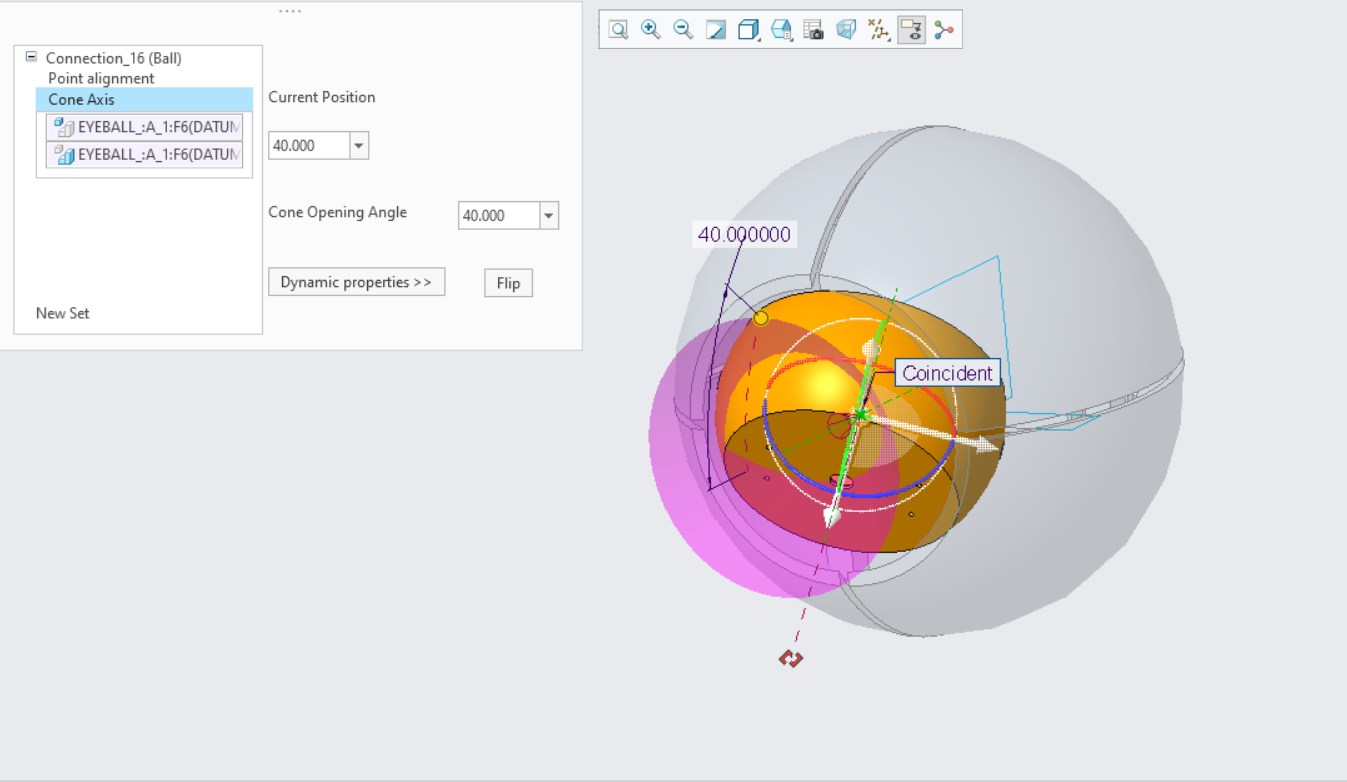
\includegraphics[width=0.5\linewidth]{Thesis/ch2/analysis1.png}
    \caption{Eye range of motion analysis.}
    \label{fig:eye-rom-analysis}
\end{figure}

It was also a concern that the robot would not be balanced and potentially fall over. This is due to the top-heavy eyeball being mounted to a slender aluminum body. To test this, a center of gravity analysis was done in Creo to ensure that the design is balanced in both the forward to backward and left to right directions. In order to perform the calculation in Creo, some approximations had to be made. In Creo, one must assign each part a material with its particular density since different densities affect the mass distribution. The 3D-printed parts were all assigned PLA, while the servo motors and any metal parts were assigned a material of Stainless Steel. This was enough to give a rough approximation, dividing the assembly up into ``heavy'' and ``light'' components. Figure \ref{fig:cog_test} shows the results of this analysis. The ``X'' in the figure indicates the center of gravity. As the figure shows, the center of gravity is nearly perfectly balanced in the left to right direction, but slightly offset in the forward to backward direction. Since the robot will be rotating around the center of the platform, it is best if the sphere of the head is centered rather than the center of gravity for symmetry purposes. An offset of half an inch is adequate for keeping the model balanced, so the project proceeded with keeping the sphere of the head centered on the circular platform for symmetry.

\begin{figure}[h]
    \centering
    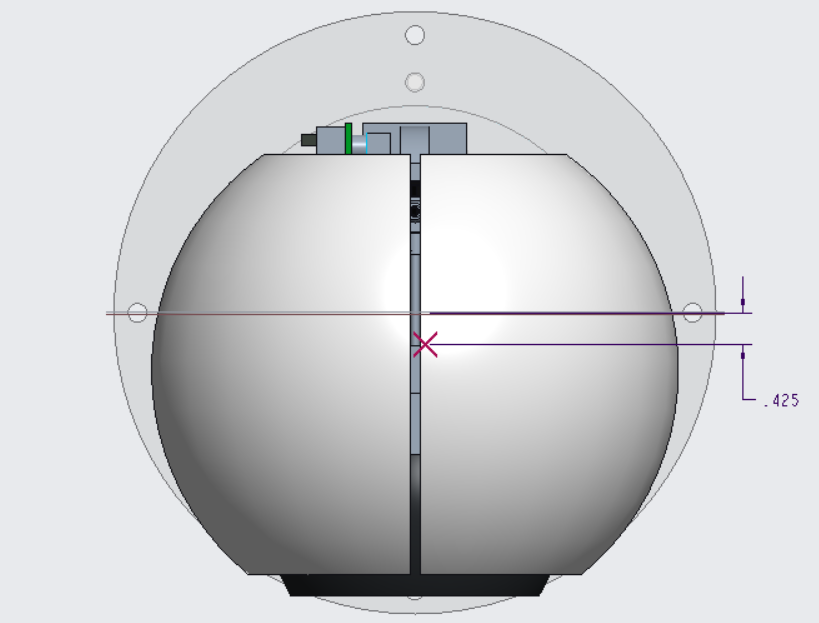
\includegraphics[width=0.5\linewidth]{Thesis/ch2/analysis2.png}
    \caption{Result of center of gravity analysis.}
    \label{fig:cog_test}
\end{figure}

\section{Finalized Model}
The final CAD model of the Mr. I robot can be seen in Figure \ref{fig:full-model}. A drawing for the overall dimensions of the model is shown in Figure \ref{fig:full-model-drw}. Note that the dimensions provided in the model are only intended to give the reader a sense of scale of the model, and are kept minimal for clarity.

\begin{figure}[h]
    \centering
    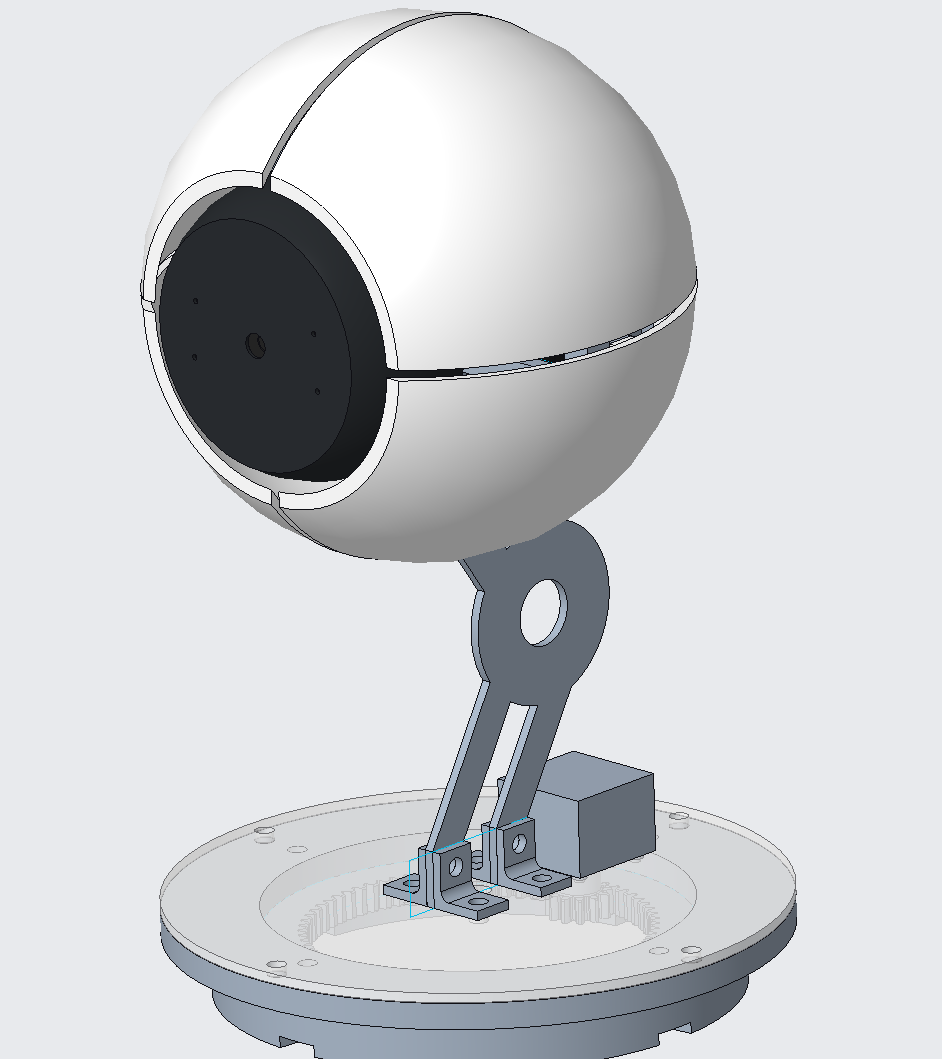
\includegraphics[width=0.4\linewidth]{Thesis/ch2/full-model.png}
    \caption{Final CAD model of the robot.}
    \label{fig:full-model}
\end{figure}
\begin{figure}[h]
    \centering
    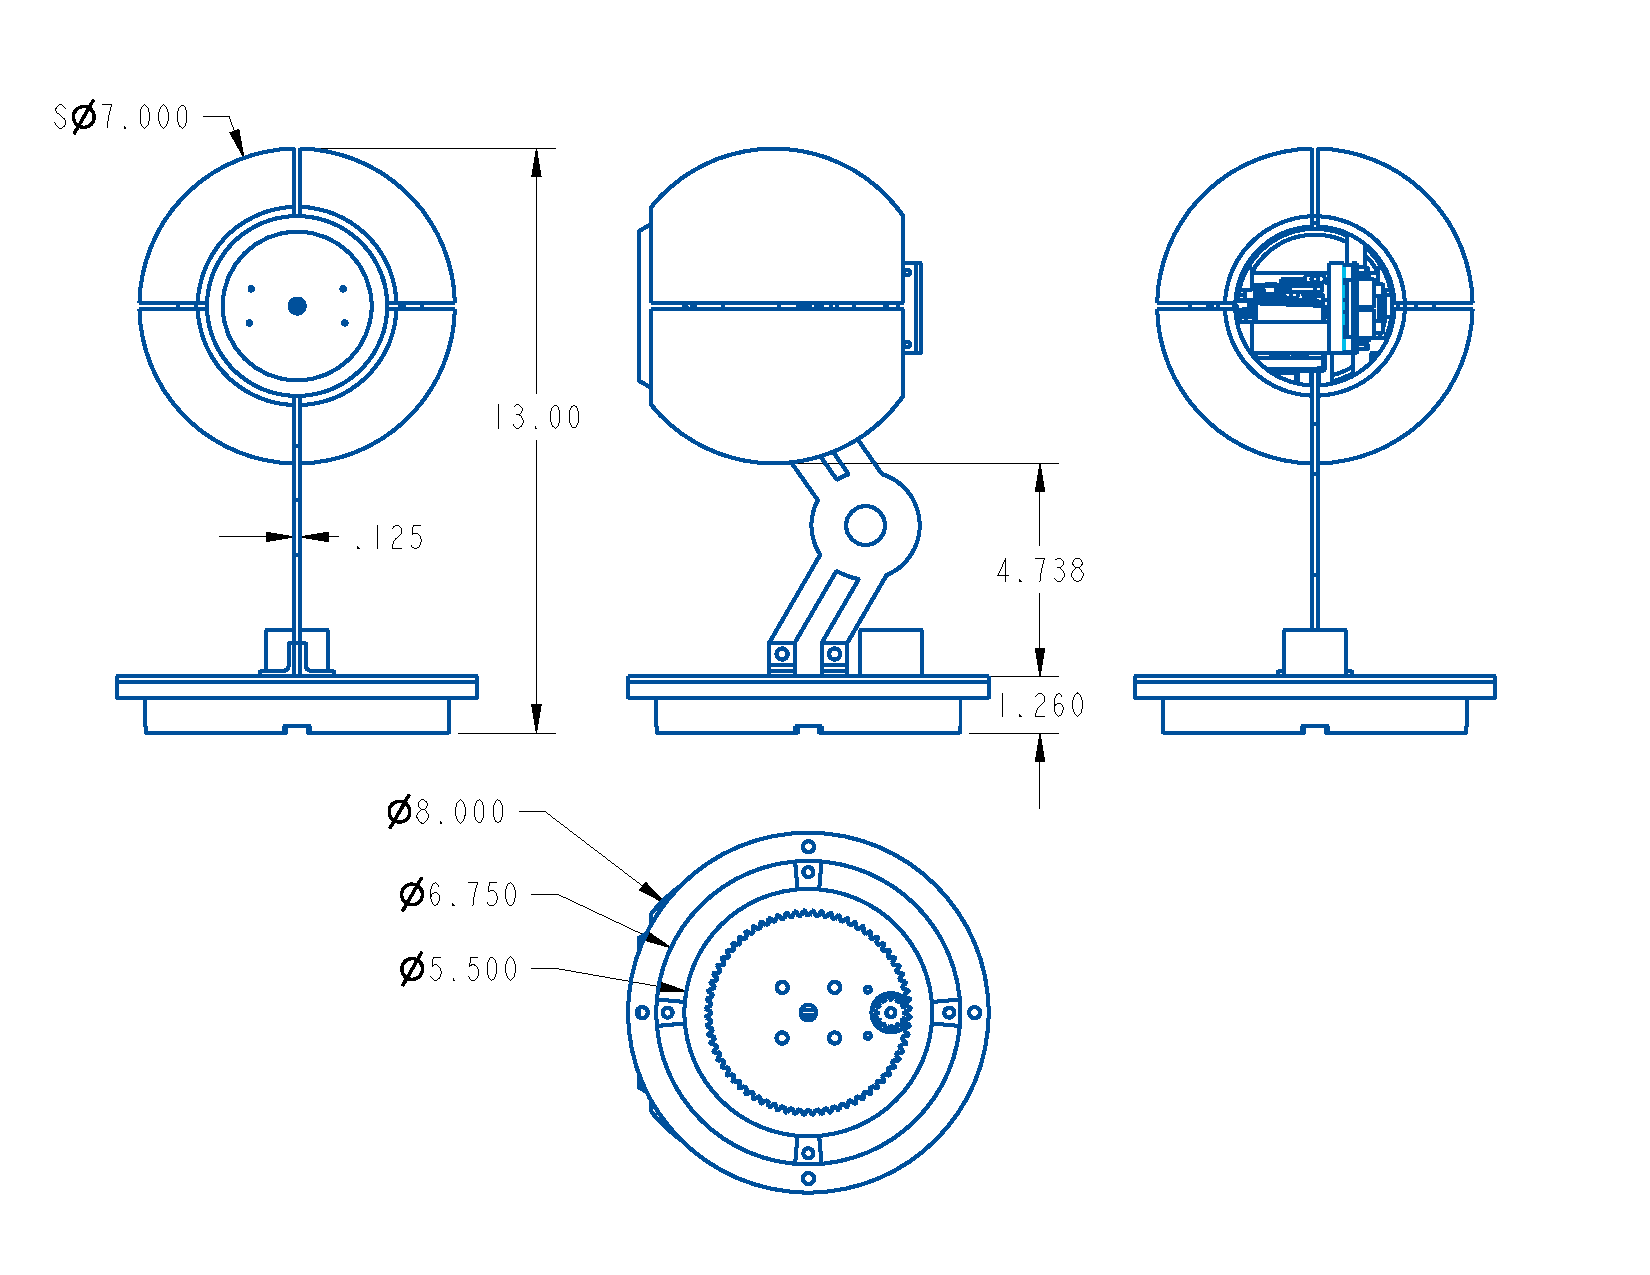
\includegraphics[width=0.8\linewidth]{Thesis/ch2/full-drw.pdf}
    \caption{Drawing of the full model.}
    \label{fig:full-model-drw}
\end{figure}